\documentclass[]{article}
\usepackage{authblk}
\usepackage{hyperref}
\usepackage{graphicx}
\usepackage{float}

\begin{document}
\title{Progressive File Transfer (PFT) Protocol}
\author{
	Jakob Buchgraber
	}

\maketitle
\tableofcontents
\newpage

\begin{abstract}
The progressive file transfer protocol (PFT) is a UDP-based protocol
that was developed for fast file transfers between a client and a
server. It supports both uploads and downloads, as well as pause
and restart of file transfers. Additionally, the protocol offers
flow control.
\end{abstract}


\section{Framing}

The frames are encoded on the wire in a framing format as specified in figure~\ref{framing}.
A PFT frame consists of a fixed 7 octet header and a variable length payload. The first
two octets specify the length of the entire frame, that is of the header and the variable
length payload. The next octet specifies the type of the frame. The last four octets of
the header specify an identifier, which uniquely identifies a connection. The identifier
is a pseudo-random non-zero byte sequence that must be chosen by the server. A server and
client is free to drop any frame with an illegal identifier i.e. zero or unknown. The variable length payload
contains the data of the specific frame type.

\begin{figure}[H]
\centering
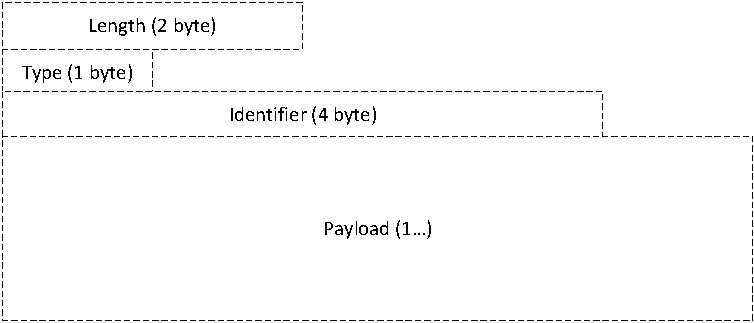
\includegraphics[width=\textwidth]{frames/framing.pdf}
\caption{Framing}
\label{framing}
\end{figure}

\section{Frames}

Subsequently we describe the format and semantics of all supported frame types. 

\subsection{Download Request}
\label{DOWNLOAD-REQ}

A client sends this frame to the server to initiate a new download
or continue a paused download. In case of a new download the SHA1
hash must be set to all zeros. For paused downloads the SHA1 hash
must be set to the hash of the whole file, as opposed to the
hash of the already downloaded data. The filename is a sequence
of US ASCII characters, where the last character must be followed
by a zero. The identifier on this frame must always be set to zero. 

\begin{figure}[H]
\centering
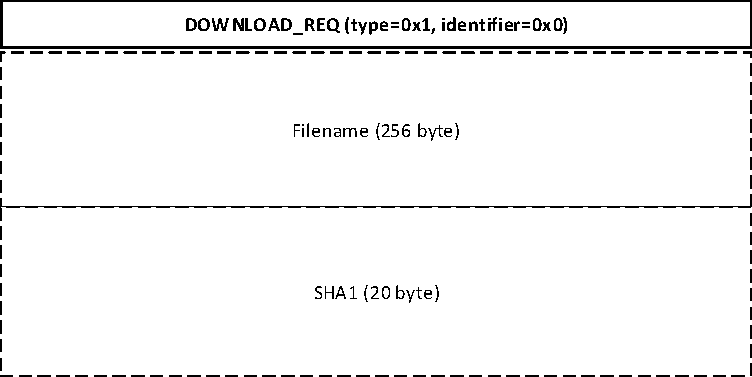
\includegraphics[width=\textwidth]{frames/download-req.pdf}
\caption{Download Request}

\end{figure}

\subsection{Download Response}

A server responds with this frame to a download request from the
client (Section~\ref{DOWNLOAD-REQ}). The frame has a random four byte identifier set, that
uniquely identifies this download. If the status is non-zero, 
then the download cannot be started. The detailed semantics of each status code are outlined
in the status code section. The port specifies on which port to
send any subsequent frames with this identifier.

\begin{figure}[H]
\centering
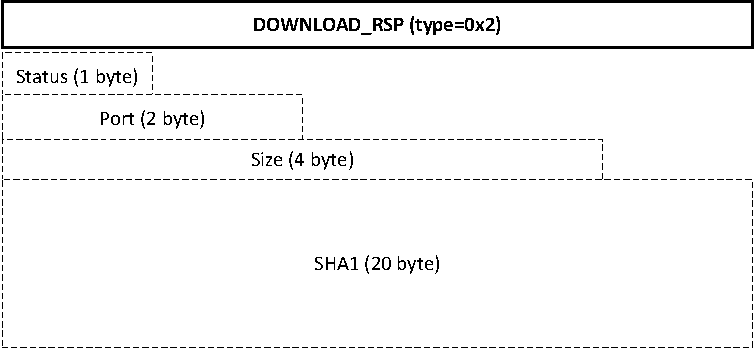
\includegraphics[width=\textwidth]{frames/download-rsp.pdf}
\caption{Download Response}
\label{DOWNLOAD-RSP}
\end{figure}

\subsection{Upload Request}
A client sends this frame to initiate a new or continue a paused upload.
The filename is a sequence of US ASCII characters, where the last character must be followed
by a zero. The SHA1 hash must be set to the hash of the whole file to be uploaded.
The size field is an unsigned integer representing the size of the whole file in bytes.

\begin{figure}[H]
\centering
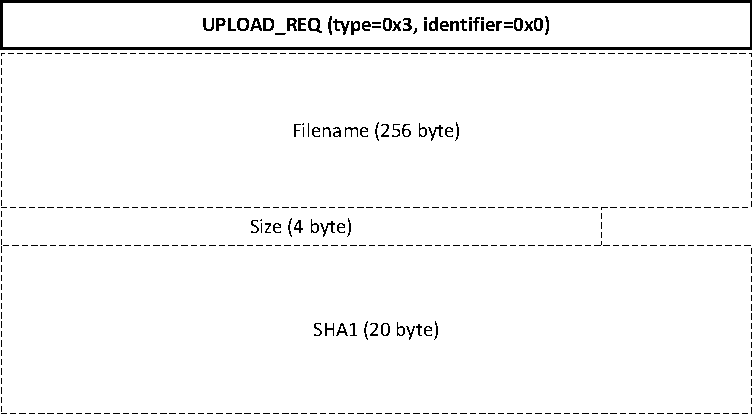
\includegraphics[width=\textwidth]{frames/upload-req.pdf}
\caption{Upload Request}
\label{UPLOAD-REQ}
\end{figure}

\subsection{Upload Response}

A server responds with thsi frame to an upload request from a client. The frame has a 
random four byte identifier set, that uniquely identifies this upload. All subsequent
frames sent for this upload by both server and client must have the same identifier set.
The port specifies on which port to send any subsequent frames with this identifier.
The upload may only begin if the status was set to OK, else the upload must be aborted
and the client must act as specified in the status section.


\begin{figure}[H]
\centering
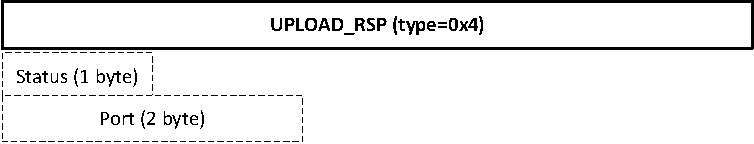
\includegraphics[width=\textwidth]{frames/upload-rsp.pdf}
\caption{Upload Response}
\label{UPLOAD-RSP}
\end{figure}

\subsection{Data Request}

In case of a download the client sends this frame to the
server, and in case of an upload the server sends this
frame to the client. This frame allows an endpoint to 
request a sequence of bytes of a given length at a specific
byte offset in a file. This frame also acts as an inbound
flow control mechanism for the receiving side. A data 
request may be answered by one or multiple data response
frames.

\begin{figure}[H]
\centering
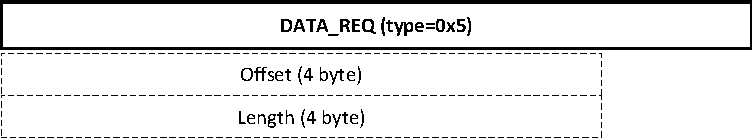
\includegraphics[width=\textwidth]{frames/data-req.pdf}
\caption{Data Request}
\label{DATA-REQ}
\end{figure}

\subsection{Data Response}

A data response frame may only be sent in response to a data request frame and
contains a sequence of bytes as requested.
Additionally it contains an offset and a length that uniquely identifies the byte sequence
within a file. That way, the order in which data response frames are received doesn't matter
either, which is an important aspect as the underlying UDP transport doesn't gurantee order.
 
\begin{figure}[H]
\centering
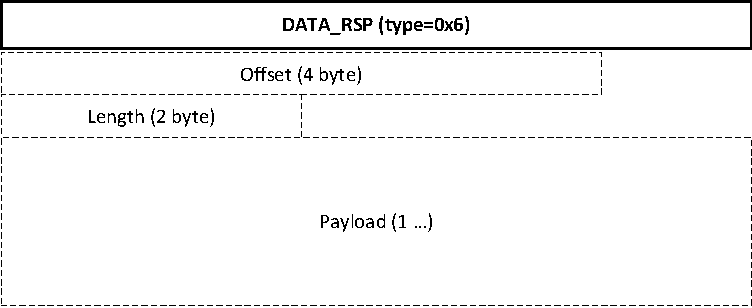
\includegraphics[width=\textwidth]{frames/data-rsp.pdf}
\caption{Data Response}
\label{DATA-RSP}
\end{figure}

\subsection{Checksum Request}
A checksum request frame may only be sent by the data receiving side. That is, by the client
in case of a download or by the server when uploading. It's used to verify the checksum of
the whole file or a part of it. It's intended to be sent after having fully received
the data of a download request, and allows to receiving side to verify the correctness early
on, as opposed to after the download or upload has finished. It may also be used to verify 
the correctness of a partially down- or uploaded file, immediately after having restarted
a down- or upload. 

\begin{figure}[H]
\centering
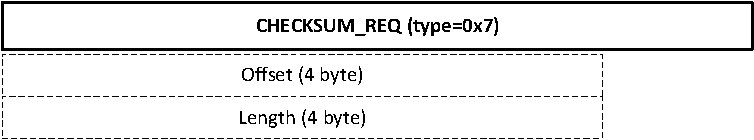
\includegraphics[width=\textwidth]{frames/checksum-req.pdf}
\caption{Checksum Request}
\label{CHECKSUM-REQ}
\end{figure}

\subsection{Checksum Response}
A checksum response frame is sent in response to a checksum request frame. It contains the SHA1
hash of the length bytes at offset. 

\begin{figure}[H]
\centering
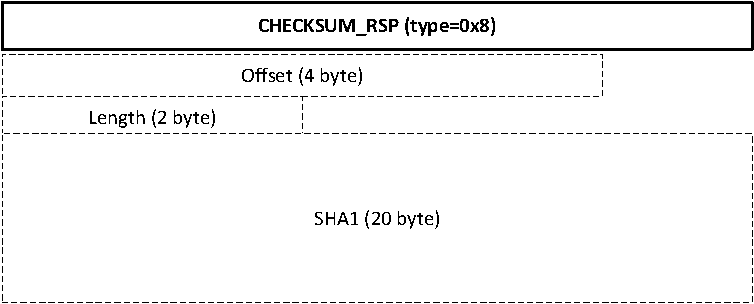
\includegraphics[width=\textwidth]{frames/checksum-rsp.pdf}
\caption{Checksum Response}
\label{CHECKSUM-RSP}
\end{figure}

\subsection{Termination Request}

This frame can be send bei either side of an upload and
download and at any point in time. After receiving
a termination request frame an endpoint needs to make a best
effort to stop any communication for the given identifier.
Any frames received after a termination request may be dropped.

\begin{figure}[H]
\centering
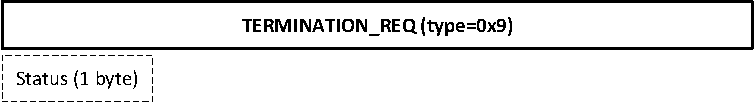
\includegraphics[width=\textwidth]{frames/shutdown-req.pdf}
\caption{Termination Request}
\label{TERMINATION-REQ}
\end{figure}

\section{Status Codes}

\begin{itemize}
\item[\textbf{OK (0x0)}] There were no errors and everything went as expected. 
\item[\textbf{ERROR (0x1)}] Something went wrong.
\item[\textbf{RETRY (0x2)}] The download or upload should be retried a later point with a new upload or download request.
\end{itemize}

\newpage

\section{Example Download}
This interaction diagram shows how a client might download a 16KB text file from a server.

\begin{figure}[H]
\centering
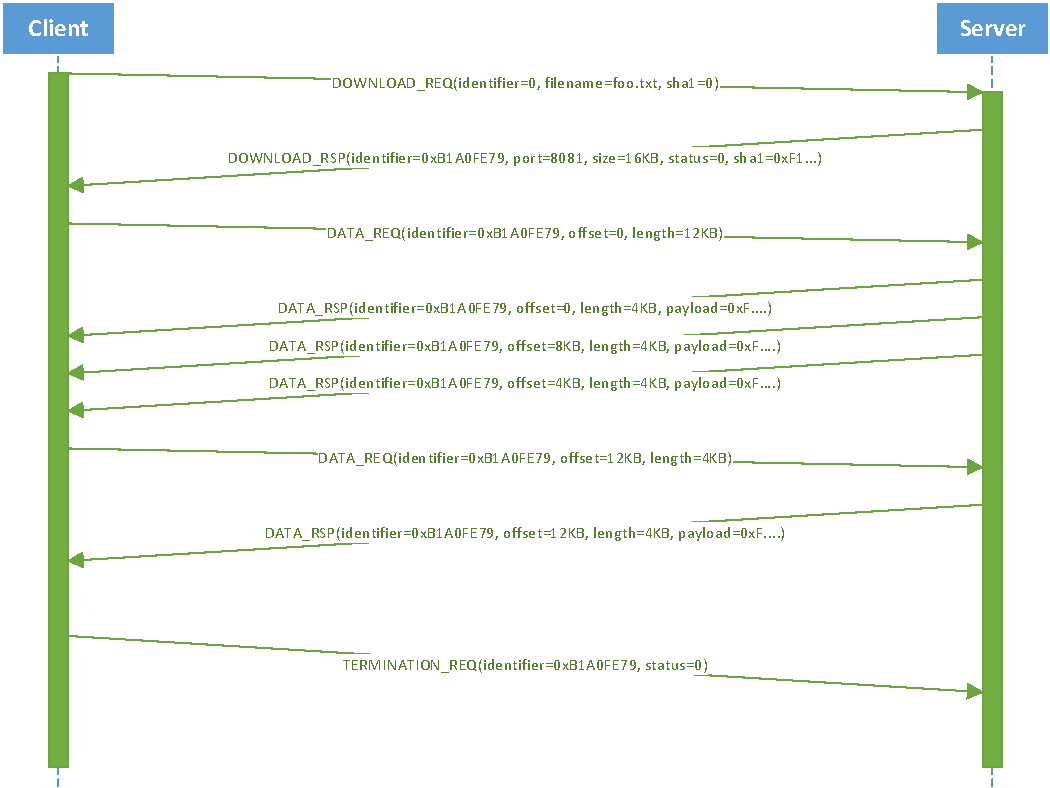
\includegraphics[width=\textwidth]{frames/download-interaction.pdf}
\caption{Example Download}
\label{EXAMPLE-DOWNLOAD}
\end{figure}


\end{document}
